\chapter{Signal Reflection}
    \section{Định nghĩa Phản xạ tín hiệu (Signal Reflection)}
        \subsection{Hiện tượng phản xạ\cite{allaboutcircuits_reflection}\cite{cadence2021reflection}}
            Phản xạ, khúc xạ, nhiễu xạ, và giao thoa - tất cả các hiện tượng cửa sóng cổ điển
            đều áp dụng cho bức xạ điện từ. Trong chương hiện tại, chúng ta chỉ quan tâm đến
            tín hiệu điện trong mạch, chưa được antenna chuyển đổi thành bức xạ điện từ, do đó
            chúng ta sẽ chỉ đề cập đến sự phản xạ và giao thoa của tín hiệu.\par

            \begin{figure}[h]
                \centering
                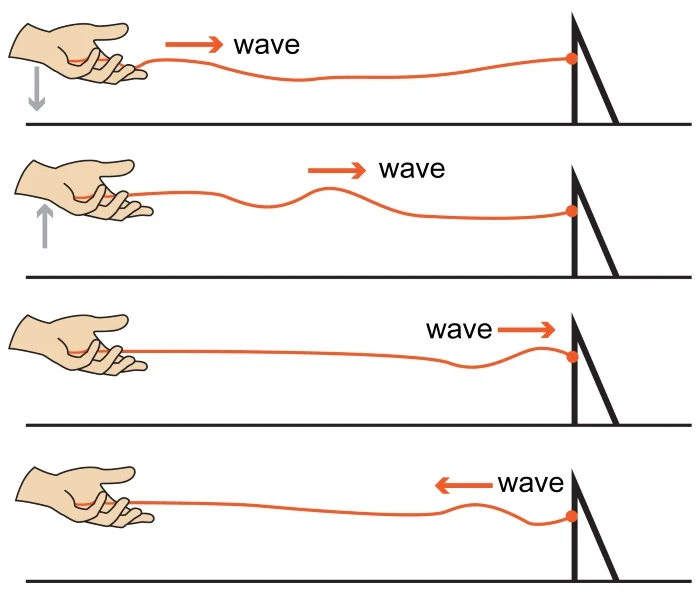
\includegraphics[width=0.5\textwidth]{figures/reflection_interference.png}
                \caption{The wave traveling along the string experiences reflection when it reaches a physical barrier.}
            \end{figure}

            Hiện tượng phản xạ xảy ra khi một sóng gặp phải một vật cản không hấp thụ sóng, hoặc hấp thụ một phần năng lượng,
            phần còn lại sẽ bị phản xạ trở lại. Tương tự trong bức xạ điện từ, vật cản ở đây chính là các thành phần điện tử trên mạch,
            với thông số gây ra sự phản xạ là trở kháng (impedance), thước đo cho mức độ cản trở dòng điện.

            Tín hiệu điện trong thực tế không truyền một chiều từ nguồn đến tải,
            mà còn có sự phản xạ ngược lại. Hay nói rõ hơn, trên một đường dẫn tín hiệu,
            tồn tại tín hiệu truyền cả hai hướng: từ nguồn đến tải, và tín hiệu phản xạ ngược lại từ tải đến nguồn.\par

            Hiện tượng này gây ra các hiệu ứng bất lợi khi sóng phản xạ có thể làm suy hao tín hiệu, thậm chí làm sai lệch và gây nhiễu,
            đặc biệt là khi thiết kế mạch truyền tín hiệu ở tần số cao như mạch RF,
            gây ra thất thoát năng lượng, nhiễu điện từ, và làm giảm đáng kể hiệu suất của mạch.

        \subsection{Xử lý hiện tượng phản xạ tín hiệu}
            Để xử lý hiện tượng phản xạ tín hiệu, cần phải hạn chế tín hiệu có thể bị phản xạ trở lại.
            Trở kháng là mức độ cản trở dòng điện, là yếu tố gây ra sự phản xạ tín hiệu.
            Để giảm sự phản xạ, cần phải giảm sự ảnh hưởng của trở kháng.
            Theo Định lý công suất cực đại\footnote{Mục \ref{sec:max_power_transfer_theorem}: Định lý công suất cực đại - Maximum Power Transfer Theorem}, 
            công suất cực đại đạt được khi độ lớn trở kháng của tải bằng độ lớn trở kháng của nguồn (đề cập đến trở kháng đặc trưng của đường truyền).
            Với trở kháng phù hợp, sẽ không có sự gián đoạn, tải có thể hấp thụ toàn bộ năng lượng của tín hiệu.\par

            Lượng năng lượng phản xạ bị ảnh hưởng bởi mức độ nghiêm trọng của sự không phù hợp trở kháng.
            Hai trường hợp xấu nhất là hở mạch (trở kháng vô cùng lớn) và ngắn mạch (trở kháng vô cùng nhỏ), 
            cả hai trường hợp này đều khiến cho toàn bộ năng lượng bị phản xạ.\par

            
    \section{Hệ số phản xạ (Reflection Coefficient)}
        \begin{figure}[h]
            \centering
            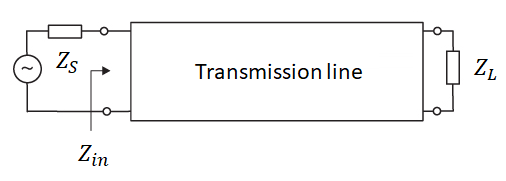
\includegraphics[width=0.5\textwidth]{figures/transmission_line.png}
            \caption{Transmission line schematic with input, source, and load impedances.}
        \end{figure}
        Hệ số phản xạ $\Gamma$\cite{cadence2023sparams}\cite{cadence2021transmission} biểu thị \textbf{mức độ sóng phản xạ lại} khi đi qua một giao diện có sự \textbf{không phù hợp trở kháng}\par
        
        \subsection{Hệ số phản xạ tại đầu tải}
            $$\Gamma_L = \frac{Z_{L} - Z_0}{Z_{L} + Z_0}$$
            \begin{itemize}
                \item $Z_{L}$: Trở kháng của tải (Load impedance)
                \item $Z_0$: Trở kháng đặc trưng của đường truyền
                \item $|\Gamma|$: Hệ số phản xạ, nằm trong khoảng $\left[0,1\right]$, giá trị càng lớn thì phản xạ càng cao
            \end{itemize}
        
        \subsection{Hệ số phản xạ tại nguồn}
            Phản xạ tại nguồn khi tín hiệu quay ngược về phía đầu vào của đường truyền:
            $$\Gamma_S = \frac{Z_{in} - Z_S}{Z_{in} + Z_S}$$
            \begin{itemize}
                \item $Z_{in}$: Trở kháng đầu vào của đường truyền
                \item $Z_S$: Trở kháng của nguồn
            \end{itemize}

        \begin{figure}[h]
            \centering
            \includegraphics[width=0.75\textwidth]{figures/signal_reflection_simulation.png}
            % \caption{Reflection coefficient at the load and source ends of a transmission line.}
        \end{figure}
        \begin{figure}[h]
            \centering
            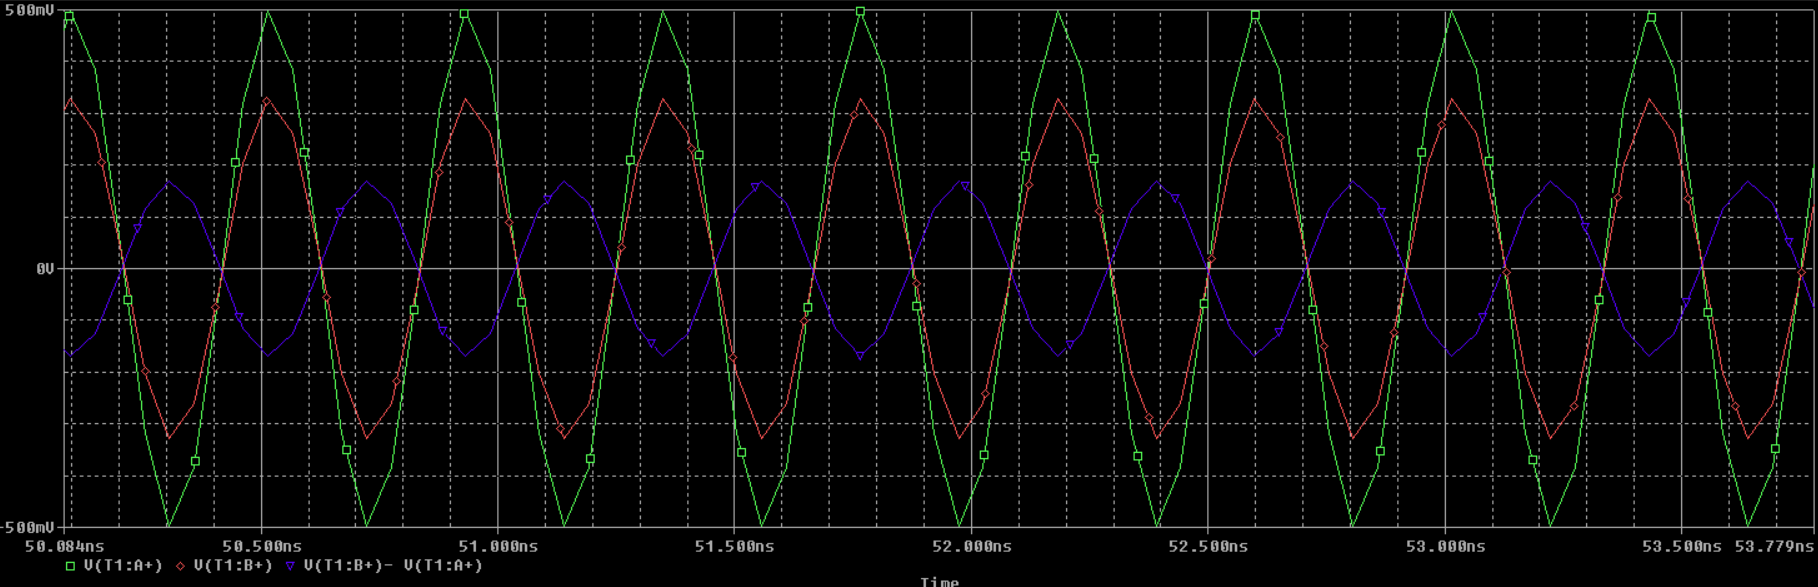
\includegraphics[width=0.75\textwidth]{figures/signal_reflection_simulation_25.png}
            % \caption{Reflection coefficient at the load and source ends of a transmission line.}
        \end{figure}
        \begin{figure}[h]
            \centering
            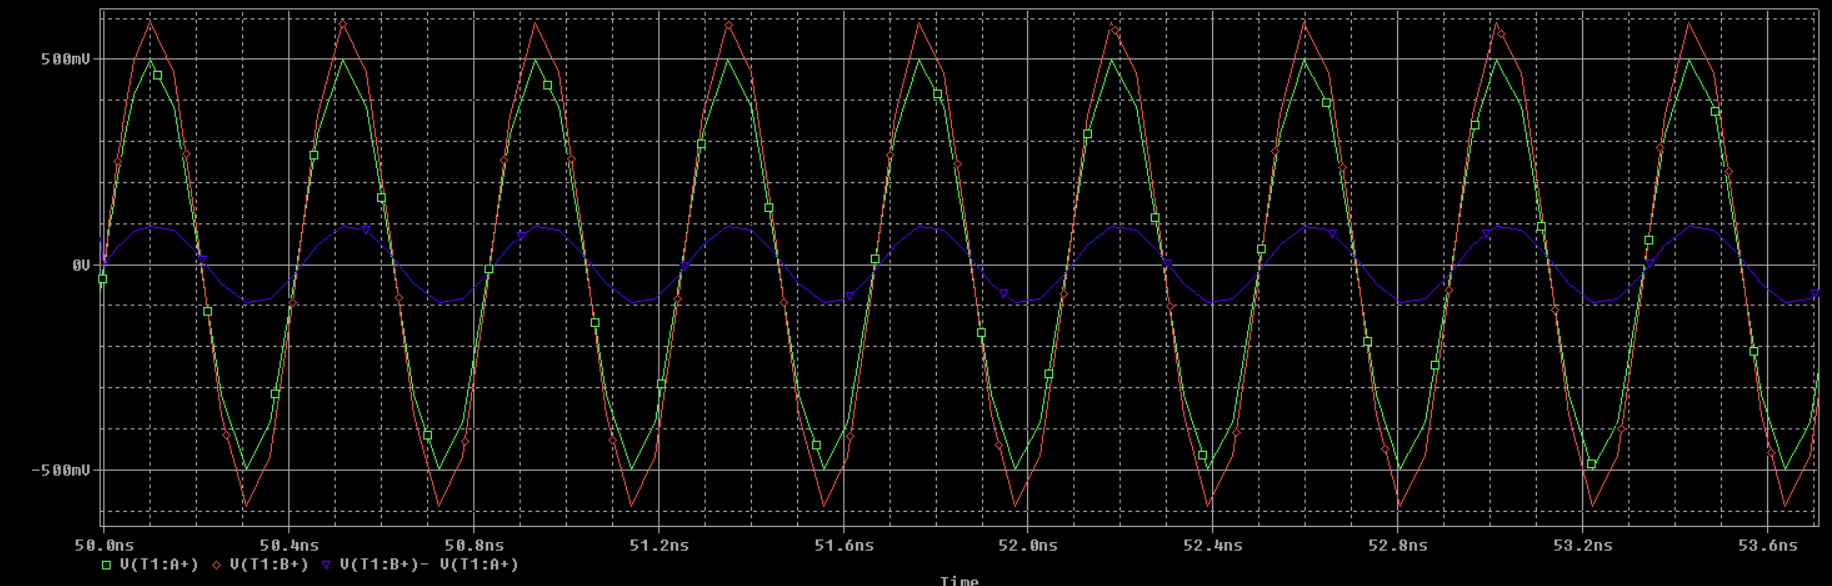
\includegraphics[width=0.75\textwidth]{figures/signal_reflection_simulation_75.png}
            % \caption{Reflection coefficient at the load and source ends of a transmission line.}
        \end{figure}\begin{figure}[h]
            \centering
            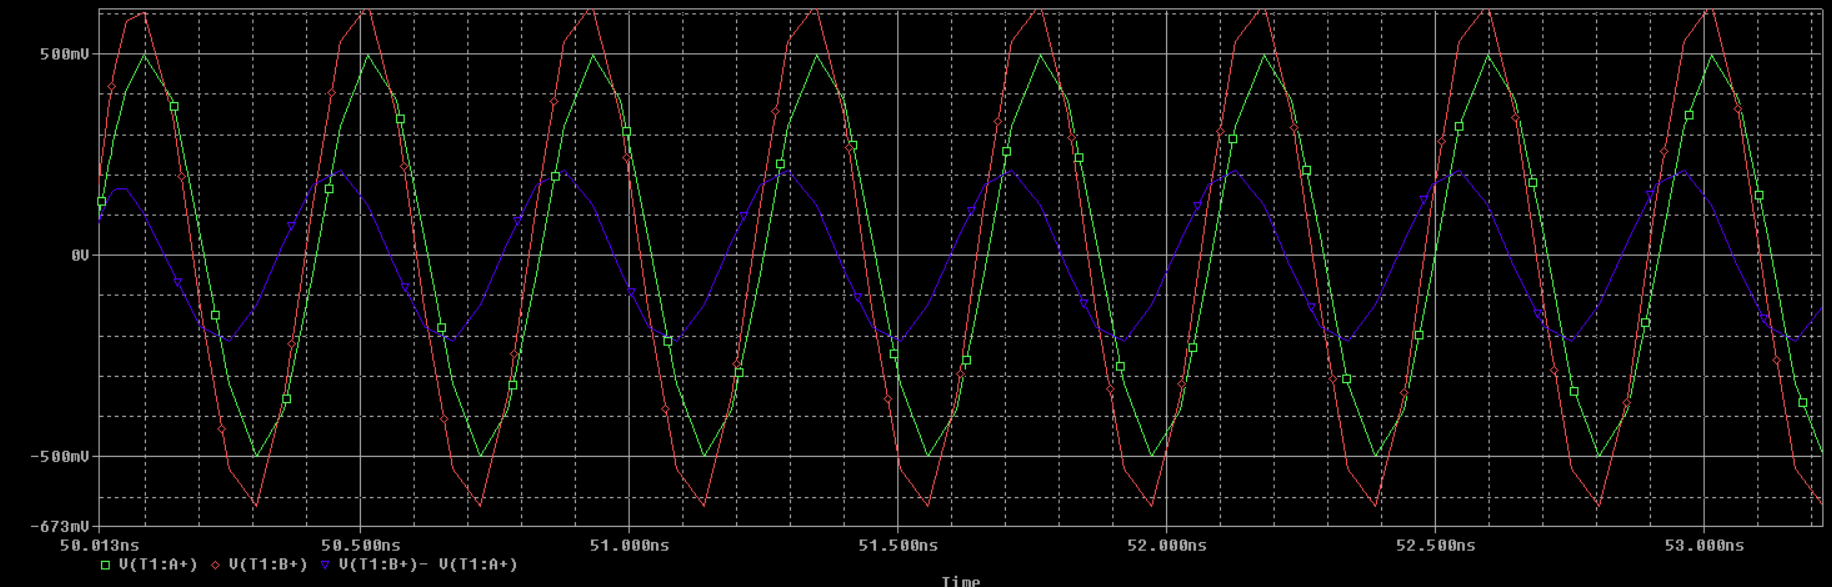
\includegraphics[width=0.75\textwidth]{figures/signal_reflection_simulation_50_33.png}
            % \caption{Reflection coefficient at the load and source ends of a transmission line.}
        \end{figure}
